\section{Methodology}

Our research has been conducted following a \textit{research in the wild} approach, meaning that we have gone out of the laboratory, and performed our investigations directly in a real setting \cite{Chamberlain2012}. More specifically, we attended two festivals in Denmark during the summer of 2018, where we were deployed our Wi-Fi sensors. During the festival (including construction/deconstruction) we have generated quantitative as well as qualitative data. We have generated quantitative data through collecting anonymized tracking data from the Wi-Fi sensors. Qualitative data has been generated through our own notes, and experiences from setting up, running, and taking down the prototyping equipment.

\subsection{Technology Use} \label{technology use}
Technically, we have used off-the shelf hardware combined with state-of-the-art software components to develop sensors and collect data. Throughout the article we use the terms \textit{device} and \textit{sensor} for describing two different elements in our setup. Device refers to external sources such as mobile phones and laptops (the entities we are tracking). Sensor refers to our hardware (trackers) we deployed during the festivals (the entities that collect data from devices).

To physically collect MAC addresses of devices, we utilized Raspberry Pi’s with an external omnidirectional Wi-Fi antenna and 4G dongles for connectivity. The external Wi-Fi antenna was a D-Link 150 High-Gain USB Adapter, which has been tested to be able to gather MAC addresses in a radius of 40 meters in perfect conditions e.g. open fields and no interference. We used a mix of Raspberry Pi 2 and Raspberry Pi 3 models, both running Raspbian, and on both models we used the same software packages. For transmitting the data, a Huawei E3372h 4G dongle was used to provide connectivity to our server where analysis was conducted. The software running on the Raspberry Pi’s was a combination of Node.js and bash commands. We utilized the TCPDump \cite{tcpdump} command available in Raspbian OS with certain flags to put the Wi-Fi interface in monitor mode and only look at the probe requests.

To comply with the current legalistic standards in Denmark \cite{blip}, the MAC addresses were put through a SHA256 hash function, which renews the salt every 24 hours at 2 a.m., to ensure that the data cannot be used to track people over multiple days. The second responsibility of the software was to normalize the data before sending it to the server. This included a dBm value, a timestamp, the hashed MAC address as well as a flag indicating if a given mobile devices is spoofing it’s MAC address, using the 7’th bit in the OUI octet of the MAC address. The latter gives us the possibility to distinguish between spoofed and non-spoofed devices, or universally administered addresses (UAA) and locally administered addresses (LAA)~\cite{spoofing}.

\subsection{Data processing} \label{sec:dataproc}
The collected data went through pre-processing to reduce noise, filter out irrelevant data, anonymize data and perform feature extraction prior to the data analysis. The first pre-processing steps include restricting the data to the festival interval (from 3 a.m. of the first day to 2 a.m. of the day after the festival), removing data created by the Wi-Fi antennas of our sensors and round the timestamps to 30 seconds. Since there can be multiple datapoints for the same device at the same timepoint, we use the one with the dBm closest to zero, i.e. closest to the device whose signal was recorded.

We can use this data to count how many devices have been seen at a defined time-interval (not smaller than 30 seconds) and location and visualize it in form of a timeline. However, when looking at movement of visitors, we need to remove spoofed data, data from stationary devices and other spurious data. Therefore, and since we were interested in information about every device, i.e. visitor, we extracted features for every unique hash, i.e. device, similarly to~\cite{largescalemonitoring}: 1) The time a device was at the festival. This is computed by the difference of the timestamp of first and last record of this device ignoring intervals without a record, larger than or equal to 2 hours. 2) Number of unique sensors a device has been seen at 3) Number of times a device has switched between sensors 4) Whether the device was seen in a restricted area, where only employees and volunteers have access.

\subsection{Data filtering} \label{sec:filtering}

\begin{figure}[tb]
  \centering
  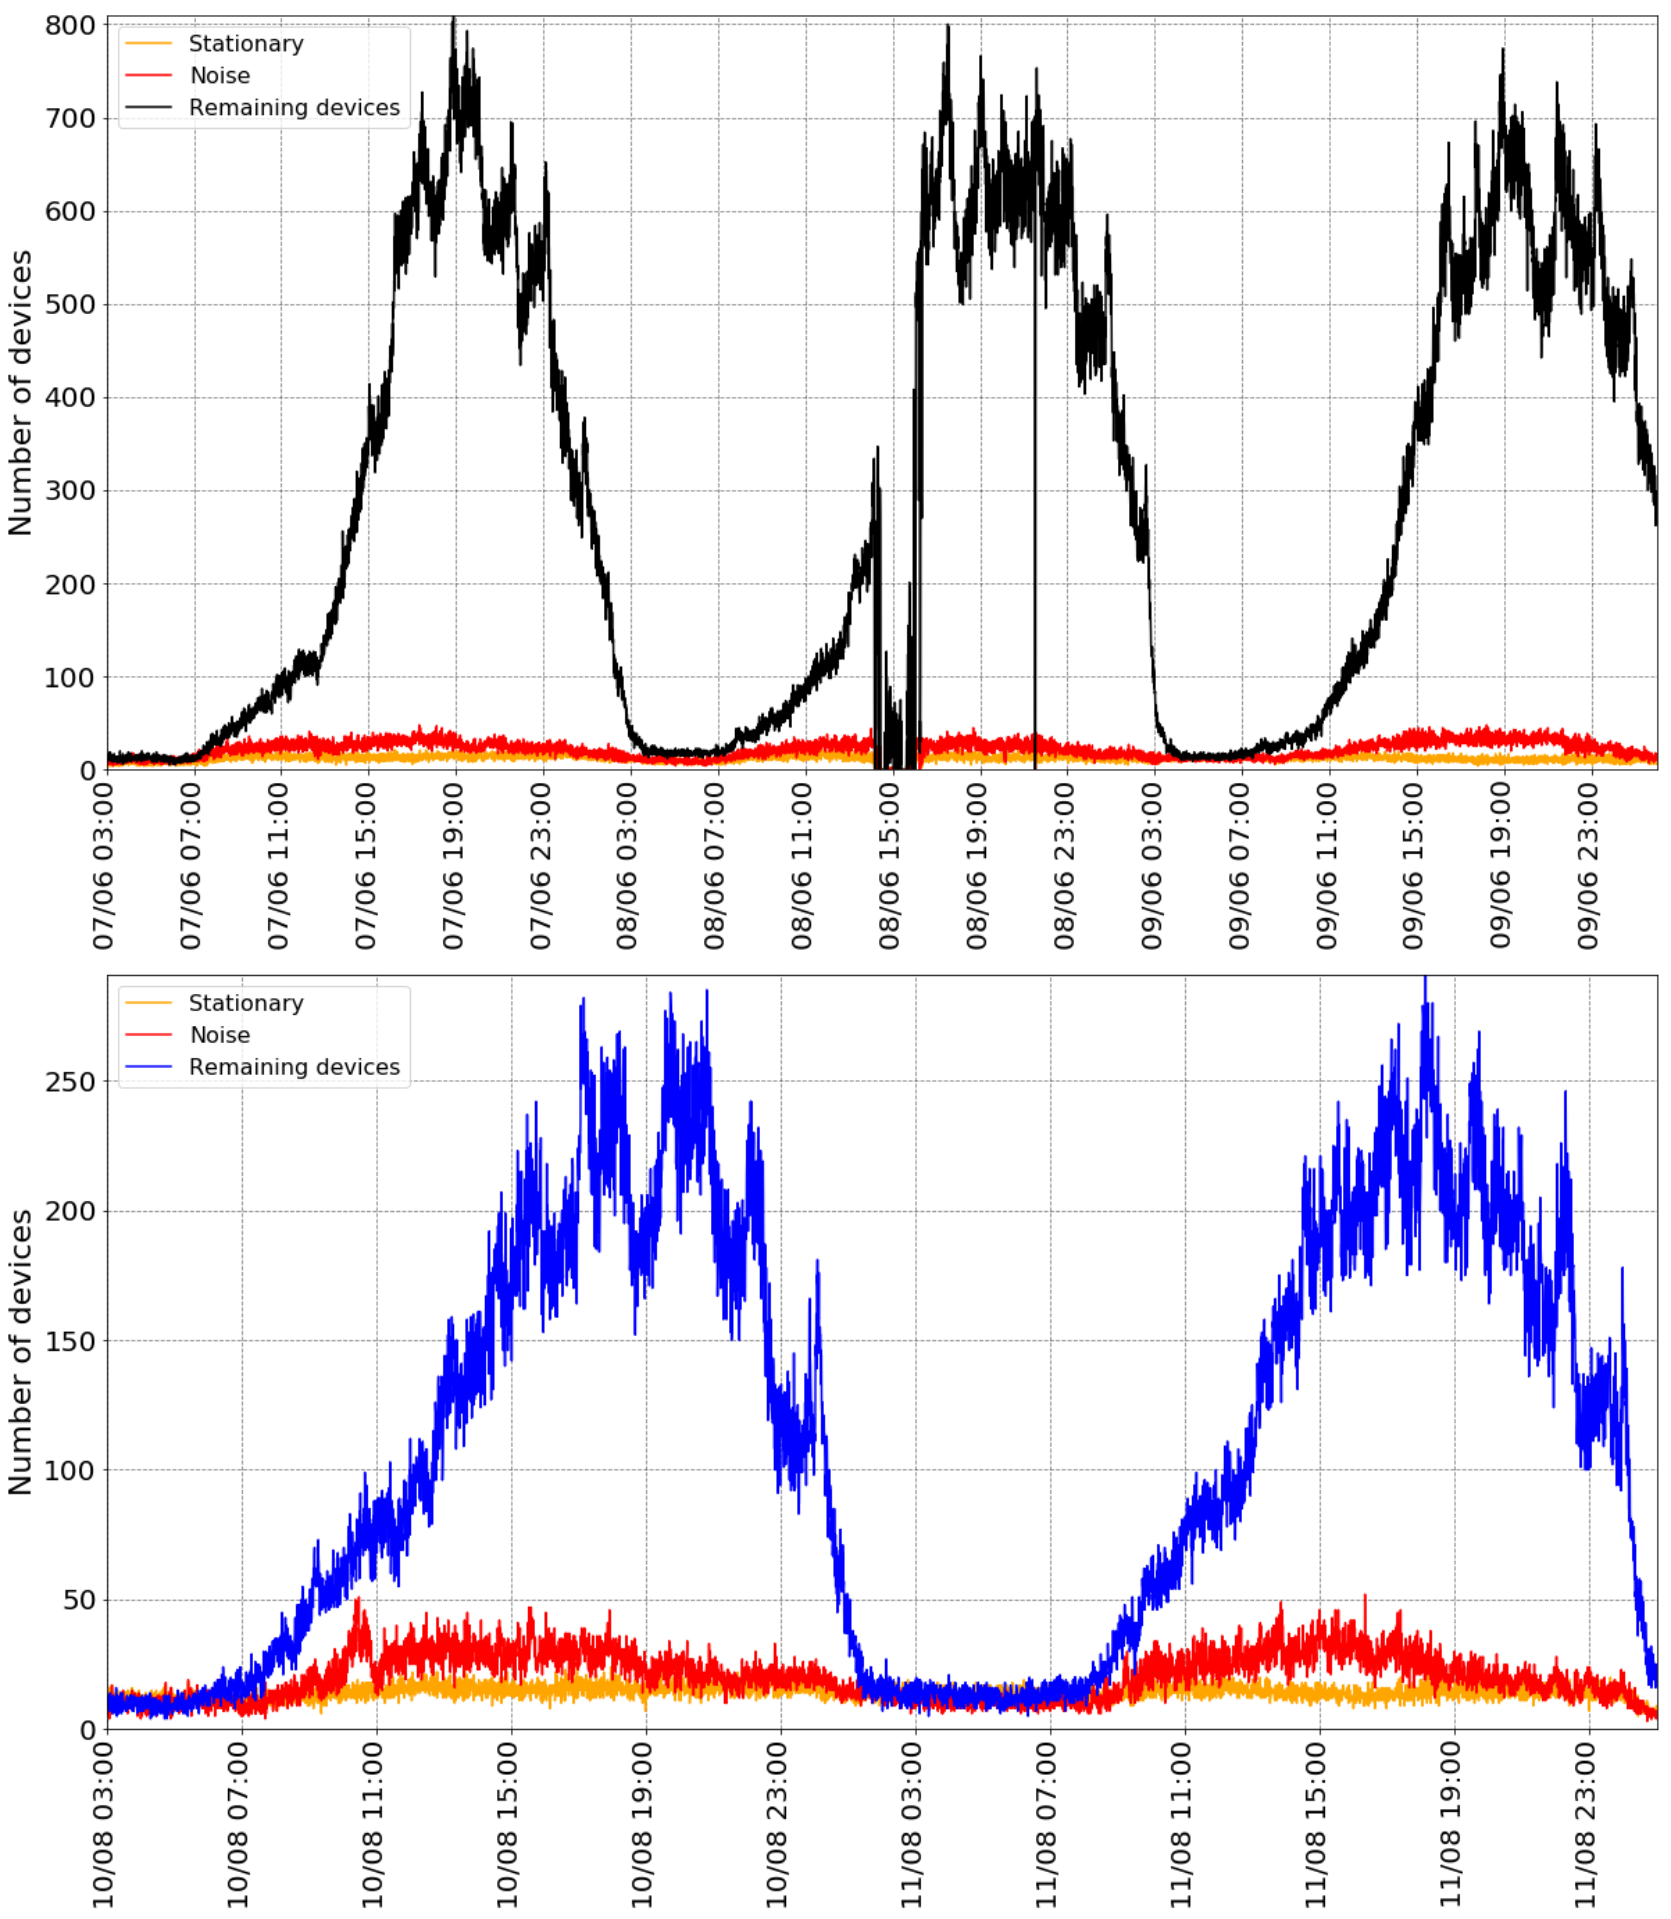
\includegraphics[width=\linewidth]{figs/stationary_noise.png}
  \caption{Number of stationary devices (orange), devices considered noise (red) and remaining devices (Northside: black, Haven: blue) as timeline over the festival days in 30 second steps. Stationary devices were tagged based on number of sensors they have been seen at ($<3$) and number of hours they where at the festival ($>14$). Noise devices were tagged based on number of sensors they have been seen at ($<3$) or number of minutes they where at the festival ($<5$).}
  \label{fig:stationary_noise}
\end{figure}

It is necessary to remove data that was recorded from signals sent by stationary devices, so that only signals from mobile devices are kept. Stationary devices that can be present at the festival are laptops used by the employees or volunteers, Wi-Fi access points or mobile phones of employees and volunteers located at the same place (typically entrance or food/drink booth) for several hours.  

Unlike~\cite{largescalemonitoring} we do not have access to the MAC address, but only to a hash. We can therefore not use it to filter devices based on the hardware producer. Instead we used an approach similar to~\cite{monitorflows}. We assume that devices seen at few sensors ($<n_{stat}$) and for a long period of time ($>t_{stat}$) are stationary. Note that using $n=1$ can be too small if the granularity is fine enough for a stationary device constantly being recorded by multiple sensors.

In addition to stationary devices, many devices are only seen at few sensors ($<10\%$ of the total amount of sensors) or only for a short period of time (only a couple of minutes). It is questionable that this data can be used to learn something about the movement of visitors. We therefore decided to remove devices which have been seen at less than $n_{noise}$ sensors or for less than $t_{noise}$ minutes.

We chose the following settings: $n_{stat}=n_{noise}=3$, $t_{stat}=14$ hours, and $t_{noise}=5$ minutes.
These were selected after a visual inspection of timeline graphs showing the number of devices over time (see Figure~\ref{fig:stationary_noise}) for a set of chosen values for $n_{stat}$, $n_{noise}$, $t_{stat}$ and $t_{noise}$, so that the amount of stationary and noise devices is approximately constant~\cite{largescalemonitoring} and a reasonable amount is filtered out. Values for this grid search were based on ad-hoc experience.